%\chapter{Spin analysis for the $X\to \jpsi \phi$ and $Z_{cs}\to \jpsi K$ states}
\section{Spin and parity study}
\label{Sec:JP}

To determine the quantum numbers of each $X$ and $Z_{cs}$ state, 
fits are done under alternative $J^P$ hypotheses. 
The likelihood-ratio test is used to quantify rejection of these hypotheses. 
Since different spin-parity assignments are represented by different functions in the angular part of the fit PDF, 
they represent separate hypotheses. For two models representing separate
hypotheses, 
assuming a $\chi^2$ distribution with one degree of freedom for $\Delta(-2\ln\Like)$ under the disfavored $J^P$ hypothesis gives a lower limit on the significance of its rejection~\supercite{LHCb-PAPER-2014-014}. 
In practice, the significance for rejection of a $J^P$ hypothesis is computed as  $\sigma(J^P)=\sqrt{\Delta(-2\ln\Like)}$, 
where $\Delta(-2\ln\Like)=2\ln\Like(J^P)-2\ln\Like(\rm preferred)$, 
\ie the likelihood difference between the fits for given $J^P$ hypothesis and for the preferred $J^P$ for this state is used. 
The preferred $J^P$ corresponds to the fit returning the smallest $-2\ln\Like$. 
In order to make sure the state is the same for different $J^P$ hypotheses, mass and width are limited to be within $\pm5\sigma$ range of the nominal fit results. 
The results for the default model are shown in Table~\ref{tab:jp}, 
and for the extended-$K^*$ model in Table~\ref{tab:jpextend}. 
The $J^P$ of previous reported four $X$ states are confirmed to be correct. 
Two new exotic states $Z_{cs}(4000)$ and $X(4675)$ are determined to be both $1^+$ for more than 15\,$\sigma$ level. 
The $J^P$ of the other new exotic states are not uniquely determined. 
The broad $Z_{cs}(4220)$ $J^P$ hypothesis can be $1^+$ or $1^-$ within about $2\,\sigma$, 
therefore, both hypotheses for $Z_{cs}(4220)$ are used to test other states' $J^P$ values. 
The $X(4175)$ state prefers $2^-$ by more than $4\,\sigma$. 
The $X(4650)$ state prefers $1^-$ by $3\,\sigma$ over $2^-$ hypothesis. 
The other hypotheses are rejected by more than $5\,\sigma$.
\begin{table}[hbtp]
\centering
\caption{Statistical significance of $J^P$ preference for the $X$ and $Z_{cs}$ states in the default model. 
For the states with two lines, the upper (lower) row corresponds to the tests with $Z_{cs}(4220)$ $J^P=1^{-(+)}$. 
The bold numbers highlight $J^P$ values which cannot be ruled out with at least $5\,\sigma$ significance.}\label{tab:jp}
\begin{tabular}{lcccccc}\hline
$J^P$ & $0^{+}$& $0^{-}$ & $1^{+}$ & $1^{-}$ & $2^{+}$& $2^{-}$ \\ \hline
  $ X(4150) $ &$   \bf 4.7 \sigma$ &$   6.1 \sigma$ &$   5.9 \sigma$ &$   5.5 \sigma$ &$   \bf 4.6 \sigma$ &prefer\\
   $ X(4150) $ &$   9.7 \sigma$ &$  12 \sigma$ &$   9.6 \sigma$ &$   5.4 \sigma$ &$   9.2 \sigma$ &prefer\\
\hline
 $ X(4630) $ &$  12 \sigma$ &$  11 \sigma$ &$   9.6 \sigma$ &prefer&$   8.5 \sigma$ &$   9.1 \sigma$ \\
  $ X(4630) $ &$   8.3 \sigma$ &$   6.1 \sigma$ &$   7.3 \sigma$ &prefer&$   6.3 \sigma$ &$   \bf 4.1 \sigma$ \\
\hline
 $ X(4500) $ &prefer&$  19 \sigma$ &$  19 \sigma$ &$  18 \sigma$ &$  21 \sigma$ &$  20 \sigma$ \\
  $ X(4500) $ &prefer&$  21 \sigma$ &$  20 \sigma$ &$  19 \sigma$ &$  21 \sigma$ &$  20 \sigma$ \\
\hline
 $ X(4700) $ &prefer&$  19 \sigma$ &$  18 \sigma$ &$  19 \sigma$ &$   15 \sigma$ &$  18 \sigma$ \\
  $ X(4700) $ &prefer&$  19 \sigma$ &$  19 \sigma$ &$  19 \sigma$ &$  16 \sigma$ &$  18 \sigma$ \\
\hline
 $ X(4140) $ &$  16 \sigma$ &$  15 \sigma$ &prefer&$  16 \sigma$ &$  14 \sigma$ &$  15 \sigma$ \\
  $ X(4140) $ &$  16 \sigma$ &$  17 \sigma$ &prefer&$  15 \sigma$ &$  17 \sigma$ &$  15 \sigma$ \\
\hline
 $ X(4274) $ &$  18 \sigma$ &$  19 \sigma$ &prefer&$  18 \sigma$ &$  18 \sigma$ &$  19 \sigma$ \\
  $ X(4274) $ &$  18 \sigma$ &$  18 \sigma$ &prefer&$  18 \sigma$ &$  18 \sigma$ &$  18 \sigma$ \\
\hline
 $ X(4685) $ &$  16 \sigma$ &$  16 \sigma$ &prefer&$  16 \sigma$ &$  15 \sigma$ &$  16 \sigma$ \\
  $ X(4685) $ &$  17 \sigma$ &$  17 \sigma$ &prefer&$  16 \sigma$ &$  16 \sigma$ &$  16 \sigma$ \\
\hline
 $ Z_{cs}(4000) $ &- &$  19 \sigma$ &prefer&$  19 \sigma$ &$  18 \sigma$ &$  19 \sigma$ \\
 $ Z_{cs}(4000) $ &- &$  18 \sigma$ &prefer&$  16 \sigma$ &$  16 \sigma$ &$  16 \sigma$ \\
 \hline
 $ Z_{cs}(4220) $ &- &$  11 \sigma$ &prefer&$   \bf 2.4 \sigma$ &$   9.5 \sigma$ &$   9.1 \sigma$ \\\hline
\hline
\end{tabular}
\end{table}


\begin{table}[htbp]
\centering
\caption{Statistical significance of $J^P$ preference for the $X$ and $Z_{cs}$ states in the extended model.
For the states with two lines, the upper (lower) row corresponds to the tests with $Z_{cs}(4220)$ $J^P=1^{-(+)}$. 
The bold numbers highlight $J^P$ values which cannot be ruled out with at least $5\,\sigma$ significance.
}\label{tab:jpextend}
\begin{tabular}{lcccccc}\hline
$J^P$ & $0^{+}$& $0^{-}$ & $1^{+}$ & $1^{-}$ & $2^{+}$& $2^{-}$ \\ \hline
 $ X(4150) $ &$   6.7 \sigma$ &$   7.4 \sigma$ &$   7.4 \sigma$ &$   5.8 \sigma$ &$   \bf 4.2 \sigma$ &prefer\\
  $ X(4150) $ &$   6.6 \sigma$ &$   9.1 \sigma$ &$   7.7 \sigma$ &$   6.6 \sigma$ &$   6.7 \sigma$ &prefer\\
\hline
 $ X(4630) $ &$  12 \sigma$ &$  11 \sigma$ &$  10.0 \sigma$ &prefer&$  10 \sigma$ &$   8.8 \sigma$ \\
  $ X(4630) $ &$   6.7 \sigma$ &$   5.3 \sigma$ &$   5.8 \sigma$ &prefer&$   5.9 \sigma$ &$  \bf 3.0 \sigma$ \\
\hline
 $ X(4500) $ &prefer&$  19 \sigma$ &$  20 \sigma$ &$  18 \sigma$ &$  20 \sigma$ &$  19 \sigma$ \\
  $ X(4500) $ &prefer&$  18 \sigma$ &$  18 \sigma$ &$  18 \sigma$ &$  18 \sigma$ &$  18 \sigma$ \\
\hline
 $ X(4700) $ &prefer&$  19 \sigma$ &$  19 \sigma$ &$  19 \sigma$ &$  16 \sigma$ &$  19 \sigma$ \\
  $ X(4700) $ &prefer&$  18 \sigma$ &$  19 \sigma$ &$  18 \sigma$ &$  14 \sigma$ &$  17 \sigma$ \\
\hline
 $ X(4140) $ &$  14 \sigma$ &$  15 \sigma$ &prefer&$  20 \sigma$ &$  13 \sigma$ &$  15 \sigma$ \\
  $ X(4140) $ &$  14 \sigma$ &$  15 \sigma$ &prefer&$  14 \sigma$ &$  13 \sigma$ &$  14 \sigma$ \\
\hline
 $ X(4274) $ &$  18 \sigma$ &$  19 \sigma$ &prefer&$  18 \sigma$ &$  18 \sigma$ &$  19 \sigma$ \\
  $ X(4274) $ &$  18 \sigma$ &$  18 \sigma$ &prefer&$  18 \sigma$ &$  18 \sigma$ &$  19 \sigma$ \\
\hline
 $ X(4685) $ &$  17 \sigma$ &$  17 \sigma$ &prefer&$  17 \sigma$ &$  17 \sigma$ &$  15 \sigma$ \\
  $ X(4685) $ &$  16 \sigma$ &$  16 \sigma$ &prefer&$  15 \sigma$ &$  16 \sigma$ &$  15 \sigma$ \\
\hline
 $ Z_{cs}(4000) $ &- &$  18 \sigma$ &prefer&$  18 \sigma$ &$  17 \sigma$ &$  17 \sigma$ \\
 $ Z_{cs}(4000) $ &- &$  17 \sigma$ &prefer&$  17 \sigma$ &$  15 \sigma$ &$  16 \sigma$ \\
\hline
 $ Z_{cs}(4220) $ &- &$   8.6 \sigma$ &$   \bf 2.0 \sigma$ &prefer&$  \bf 4.9 \sigma$ &$   5.7 \sigma$ \\

\hline
\end{tabular}
\end{table}


We also show the nominal $K+5X+3X+2Z$ model with a $1^-$ $Z$ in Table~\ref{tab:fit1m} for completeness. 
The $1^-$ $Z$ has large width and is at the high mass boundary allowed in the $\Bp\to\jpsi \phi \Kp$ decay.
%%%%%%%%%%%%%%%%%%%%%%%%%%%%%%%%%%%%%%%%%%%%%%%%%%%%%%%%%%%%%%%%%%%%%%%%
\begin{table}[tbph]
\begin{center}
\caption{Fit results from  the 9K+5X+3X+2Z model with $Z_{cs}(4220)$ $J^P=1^-$. 
Significance is evaluated from the change of the $2\ln\Like$ assuming ndf to be {\bf twice} the reduction in number of free parameters when removing the component in the fit. 
The ndf is not multiply by two for the $K^*$ resonance whose mass and width are fixed.}\label{tab:fit1m}
\begin{tabular}{cccccc}
\hline
\multicolumn{2}{c}{Contribution} &Significance & \multicolumn{3}{c}{Fit results}  \\
                  &                           &                 & $M_0$ [MeV]   & $\Gamma_0$ [MeV]      & FF\%          \\
\hline \hline
   &     All $K(1^+)$    &        &    &   &  $10.8\pm2.6$          \\
$\nslj{2}{1}{P}{1}$   &  $K(1^+)$             & 6.4$\sigma$  &  $1867\pm 10 $  &  $147\pm27$  &       \\
$\nslj{2}{3}{P}{1}$   &  $K^{\prime}$($1^+$)  & 6.4$\sigma$  &  $1918\pm 14 $  &  $438\pm74$  &       \\
$\nslj{1}{3}{P}{1}$   &  $K_1(1400)$          & 6.9$\sigma$  &  &     &   $12.8\pm6.5$    \\
\hline

&     All $K(2^-)$    &        &        & &  $4.0\pm0.4$           \\
$\nslj{1}{1}{D}{2}$   &  $K_2 (1770)$   & 13.0$\sigma$       &    &    &     \\
$\nslj{1}{3}{D}{2}$   &  $K_2(1820)$    & 12.0$\sigma$       &    &    &     \\       

\hline
& All $K(1^-)$        & & & & $56.5\pm3.3$ \\
$\nslj{1}{3}{D}{1}$   &  $K^*(1680)$    & 9.5$\sigma$  &   &    &  $6.2\pm1.3$    \\  
$\nslj{2}{3}{S}{1}$   &  $K^*(1410)$    & 11.7$\sigma$   &   &    &  $35.8\pm3.9$   \\
\hline

& $K(2^+)$\\
$\nslj{2}{3}{P}{2}$   &  $K^*_2(1980)$  & 7.3$\sigma$   &  $1973\pm18 $   &   $301\pm67$   & $2.8\pm0.5$        \\  
\hline 
& $K(0^-)$\\
$\nslj{2}{1}{S}{0}$   &  $K(1460)$      & 14.3$\sigma$       &    &      & $9.4\pm0.9$    \\  

\hline 
\hline
&$X(2^-)$ & & & &   \\
  &$X(4150)$            & $4.8\sigma$ & $4176\pm 14$ & $112\pm32$   & $1.0\pm0.3$ \\
\hline
&$X(1^-)$ & & & &   \\
  &$X(4630)$            & $11.0\sigma$ & $4650\pm 23$ & $121\pm15$  & $5.5\pm1.0$ \\
\hline

 &All $X(0^+)$ & & & & $24.6\pm7.7$  \\
 &$X(4500)$           & $18.0\sigma$ & $4475\pm 3$ & $70\pm6$ &  $5.1\pm0.5$ \\
 &$X(4700)$           & $18.0\sigma$ & $4693\pm 4$ & $83\pm8$ &  $7.8\pm0.7$ \\
 &$NR_{J/\psi \phi}$  & $6.9 \sigma $& & &$18.7\pm4.3$ \\
\hline
 &All $X(1^+)$ & & & & $25.0\pm3.6$ \\
 &$X(4140)$           & $14.8\sigma$ & $4116\pm 10$ & $130\pm21$ & $18.0\pm6.8$ \\
 &$X(4274)$           & $17.3\sigma$ & $4295\pm 4$  & $53\pm5$   & $2.7\pm0.6$ \\
 &$X(4685)$           & $14.9\sigma$ & $4675\pm 9$  & $121\pm15$ & $5.7\pm1.2$ \\
\hline\hline
&$Z_{cs}(1^+)$ \\
  &$Z_{cs}(4000)$          & $18.2\sigma$ & $3989\pm 4$  & $109\pm15$  & $5.8\pm0.4$ \\
  \hline
&$Z_{cs}(1^-)$ \\
  &$Z_{cs}(4220)$          & $9.2\sigma$ & $4263\pm39$ & $468\pm126$ & $8.1\pm3.4$ \\
\hline
\end{tabular}
\end{center}
\end{table}




\section{Argand diagrams}

Further evidence for the resonant character of $Z_{cs}(4000)^+$ is shown in Figure.~\ref{fig:Argand} by demonstrating the evolution of the complex amplitude on the Argand diagram, 
obtained with the same
method as previously reported for the $Z_c(4430)^-$ state~\supercite{LHCb-PAPER-2014-014}.
The magnitude and phase have approximately circular evolution with $m_{\jpsi\Kp}$ in the counter-clockwise direction,
as expected for a resonance.

\begin{figure}[!tbh]
\centering
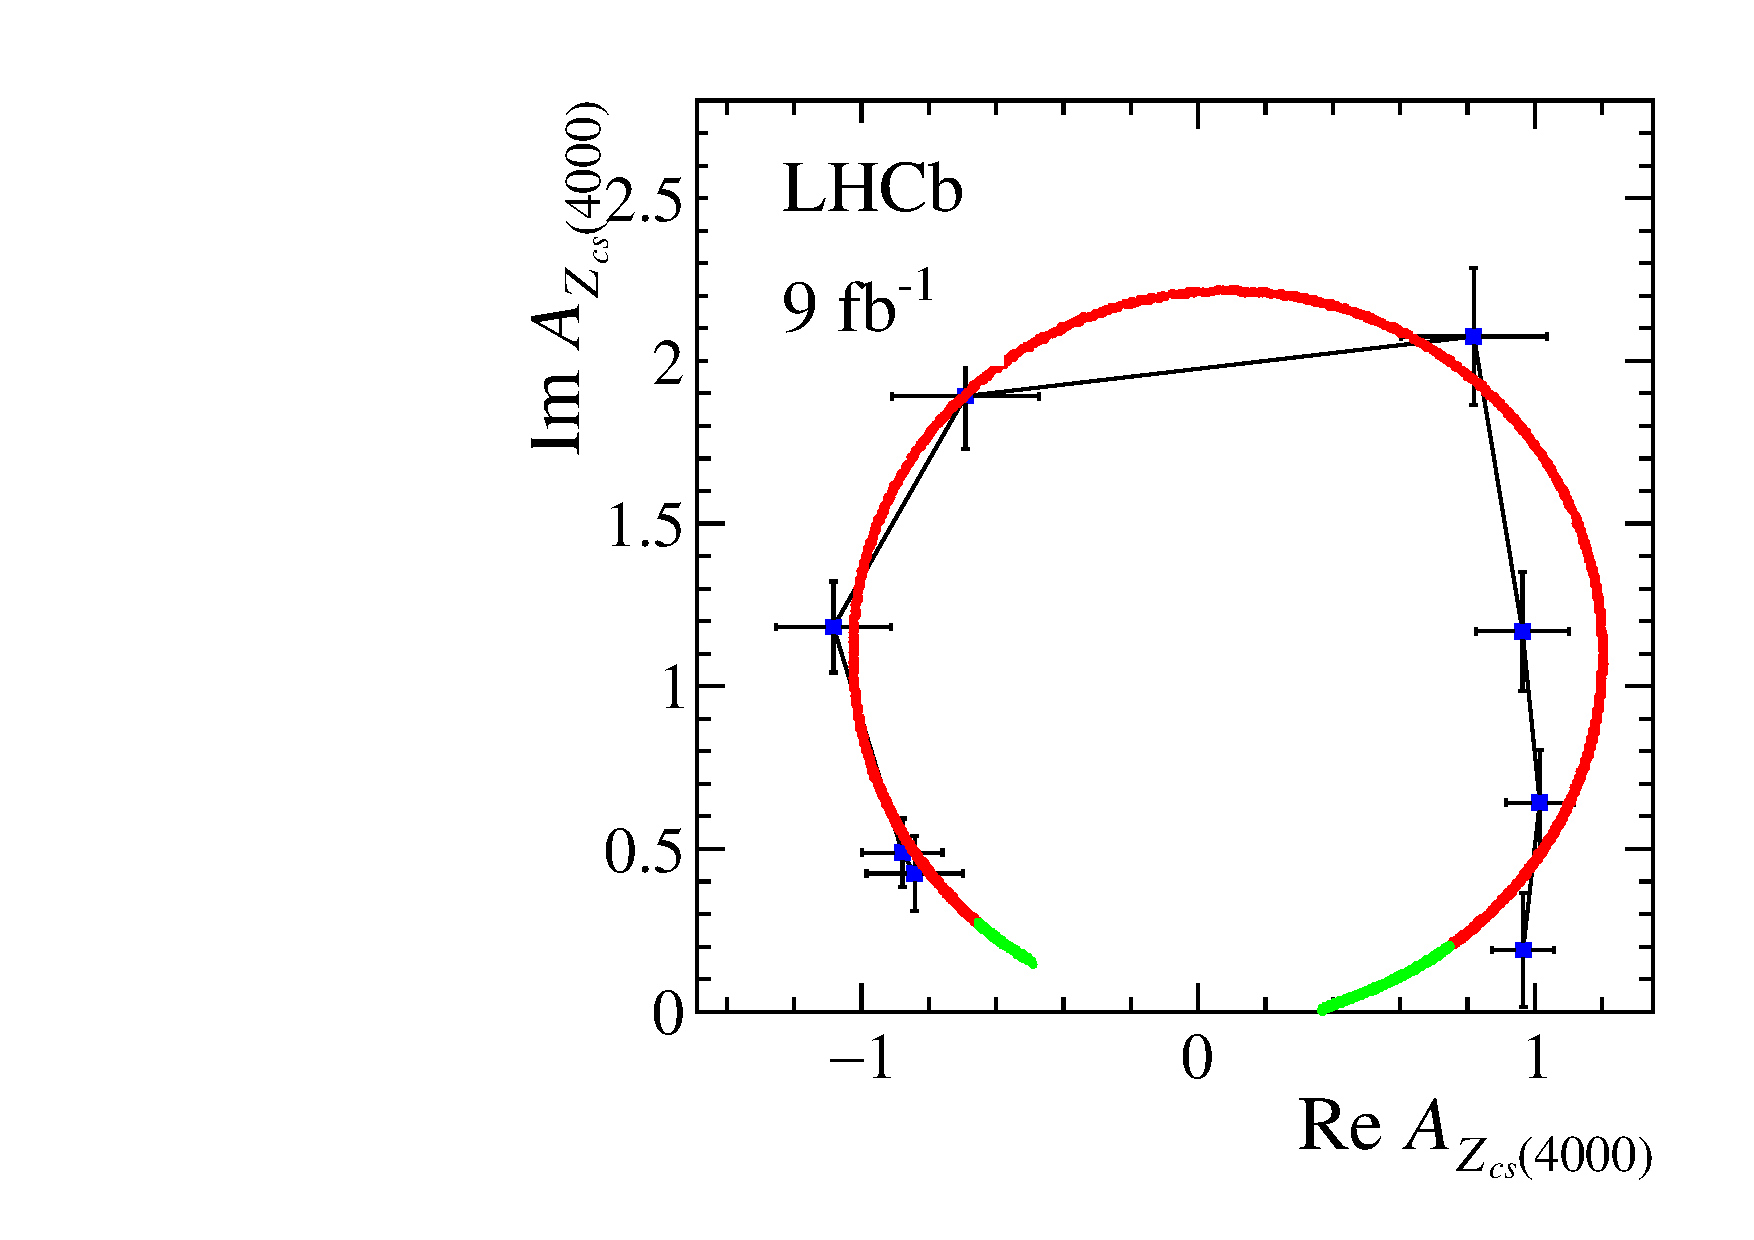
\includegraphics[width=0.6\textwidth]{Figures/03_Zcs/06_Amplitude/Z1_argand.pdf}
\caption{Fitted values of the $Z_{cs}(4000)^+$ amplitude in eight $m_{\jpsi\Kp}$ bins,
shown on an Argand diagram (blue points).
The red line represents the expected Breit-Wigner behaviour in between $-1.4\Gamma_0$ to $1.4\Gamma_0$ around the $Z_{cs}(4000)^+$ mass.
The green line is the reachable mass range in the $\Bp\to\jpsi\phi\Kp$ channel.
}
\label{fig:Argand}
\end{figure}




